\documentclass[11pt]{article}

%Afegim els "packages" necessaris per generar el document
\usepackage[utf8]{inputenc}
\usepackage{graphicx}
\usepackage{fancyhdr}
\usepackage[hidelinks]{hyperref}
\usepackage{tocloft}
\usepackage[T1]{fontenc}


\title{Instal·lació Allegro 5.1 (Linux)}
\author{Autor: Albert Lloveras Carbonell\\Revisió: Joaquim Porte Rodríguez}
\date{}

\renewcommand\contentsname{\huge Índex \vspace{8pt} \hrule}
\renewcommand{\cftsecleader}{\cftdotfill{\cftdotsep}}

%------------------------------------------------------------
%	Definició de Capçaleres i Peus de Pàgina
%------------------------------------------------------------

\fancypagestyle{pageStyle}{
	%Definim la capçalera de l'esquerra (Logo Salle)
	\fancyhead[L]{
		
\includegraphics[scale=0.25]{img/la_salle_logo.jpg}
	} 

	%Definim la capçalera de la dreta (Info Curs i Assignatura)
	\fancyhead[R]{
		\vtop{
			Manual d'instal·lació\\
			d'Allegro 5.1 (Ubuntu)\\
		}
	}
	\fancyfoot[C]{} %Peu de pàgina central
	\fancyfoot[L]{Departament d'Enginyeria - Informàtica} %Peu de pàgina esquerra
	\fancyfoot[R]{\thepage} %Peu de pàgina dreta (Número de pàgina)	
	%Configuracions extra
	\renewcommand{\headrulewidth}{0pt} %Ocultem la línia de separació entre 		capçalera i bloc de text
	\renewcommand{\footrulewidth}{2pt} %Fixem la línia de separació entre peu de pàgina i bloc de text
	\setlength{\headheight}{67pt} %Fixem la mida de la capçalera	
	
}

%Definim la macro (nofooter) per poder amagar el peu de pàgina quan interessi
\fancypagestyle{nofooter}{
	\fancyfoot{}
	\renewcommand{\footrulewidth}{0pt}
}

%Definim la macro (nofooter) per poder amagar el peu de pàgina quan interessi
\fancypagestyle{empty}{
	\fancyfoot{}
	\fancyhead{}
	\renewcommand{\footrulewidth}{0pt}
	\renewcommand{\headrulewidth}{0pt}
}

\begin{document}

\pagestyle{empty}
\begin{center}

	%--- Logo de la portada --- %
	
\includegraphics[width=0.15\textwidth]{img/allegro.png}~\\[1cm]
	
	%---- Nom del programa --- %
	\textsc{\LARGE Allegro 5.1}\\[1.5cm]
	
	%-- Nom del manual -- %
	\hrule
	\vspace{8pt}
	\huge{\bfseries Manual d'instal·lació (Ubuntu)}
	\vspace{8pt}
	\hrule	
	\vspace{12pt	}

	% -- Nom de l'autor i del supervisor
	\noindent
	\begin{minipage}{0.4\textwidth}
		\begin{flushleft} \large
			\emph{Autor:}\\
			Albert \textsc{Lloveras}
		\end{flushleft}
	\end{minipage}%
	\begin{minipage}{0.4\textwidth}
		\begin{flushright} \large
			\emph{Revisió:} \\
			Joaquim \textsc{Porte}
		\end{flushright}
	\end{minipage}
	\vfill

\end{center}

%---- Índex ---- %
\newpage

\pagestyle{empty}
\tableofcontents


%---- Començament del document --- %
\newpage
\pagestyle{pageStyle}

\section{Introducció}
En aquest manual s'explicarà com realitzar la instal·lació de la llibreria Allegro 5 a Linux per al desenvolupament d'aplicacions que requereixin d'una interfície gràfica d'usuari (GUI) com per exemple els videojocs. Cal destacar que aquesta llibreria és totalment lliure i no requereix l'adquisició de cap llicència addicional per tal de fer-ne ús en qualsevol dels nostres projectes.

\section{Obtenció del software necessari}
 Abans de començar haurem de realitzar una sèrie d'operacions per tal de posar apunt el nostre ordinador. Aquestes operacions són bàsicament la instal·lació de les llibreries addicionals de les que depèn Allegro 5 i la instal·lació de CMake per tal de poder compilar el codi font de la llibreria abans d'instal·lar-la al nostre ordinador.\\

\noindent Per començar haurem d'obrir una finestra del terminal de Linux que serà on executarem totes les comandes per tal de procedir a la instal·lació d'Allegro5. Per fer-ho, podem utilitzar la drecera de teclat \textbf{Control + Alt + T} i hauríem d'obtenir una finestra com la següent:

\begin{center}
	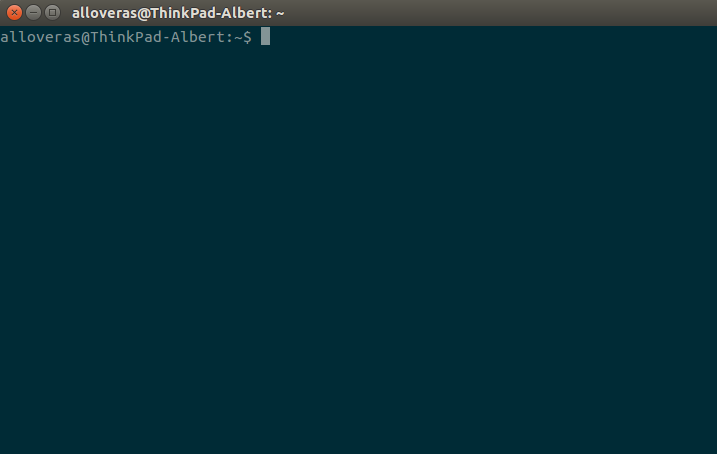
\includegraphics[scale=0.4]{img/Linux_Terminal.png}
\end{center}

\pagebreak
\noindent El primer que farem serà comprovar que tenim la versió dels repositoris d'Ubuntu actualitzats mitjançant la comanda:

\begin{center}
	\textbf{sudo apt-get update}
\end{center}

\noindent \textbf{Nota:} En totes les comandes que incloguin la directiva \textbf{sudo} se'ns demanarà la introducció de la clau d'administrador per tal de que es pugui validar que la persona que esta realitzant la instal·lació del software és l'administrador del sistema o té privilegis per realitzar la operació en qüestió.

\begin{center}
	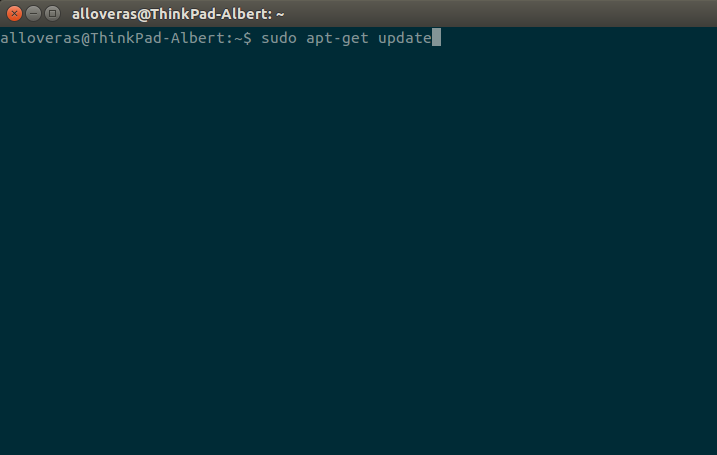
\includegraphics[scale=0.4]{img/Apt_Get_Update.png}
\end{center}

\noindent Un cop finalitzat el procés d'actualització, ja estarem llestos per realitzar la instal·lació de  les llibreries addicionals i els programes necessaris per realitzar la instal·lació. Per instal·lar tot això, farà falta executar les següents comandes amb el següent ordre:

\begin{center}
	\textbf{sudo apt-get install libgl1-mesa-dev libglu1-mesa-dev cmake build-essential make libxcursor-dev}
\end{center}

\begin{center}
	\textbf{sudo apt-get install -y cmake g++ freeglut3-dev libxcursor-dev libpng12-dev libjpeg-dev libfreetype6-dev libgtk2.0-dev libasound2-dev libpulse-dev libopenal-dev libflac-dev libdumb1-dev libvorbis-dev libphysfs-dev git}
\end{center}

\pagebreak
\noindent Arribats a aquest punt, ja estem preparats per instal·lar Allegro 5. Per fer-ho només ens farà falta obtenir-ne el codi font mitjançant la següent comanda:
\begin{verbatim}
	git clone git://git.code.sf.net/p/alleg/allegro
\end{verbatim}

\noindent La comanda anterior serveix per descarregar des del rebost de codi les fonts de la llibreria Allegro 5.1. Cal notar que els fitxers que es descarreguin es desaran a una nova carpeta \textit{allegro} que es crearà automàticament al directori al qual ens trobéssim amb el terminal quan hem executat la comanda.

\section{Instal·lació d'Allegro 5.1}
\noindent Un cop acabada a descàrrega anirem a la carpeta \textit{allegro} on hem clonat el codi movent-nos pel terminal ajudant-nos de la comanda \textbf{cd}. A continuació es mostra un exemple del procediment a seguir:

\begin{center}
	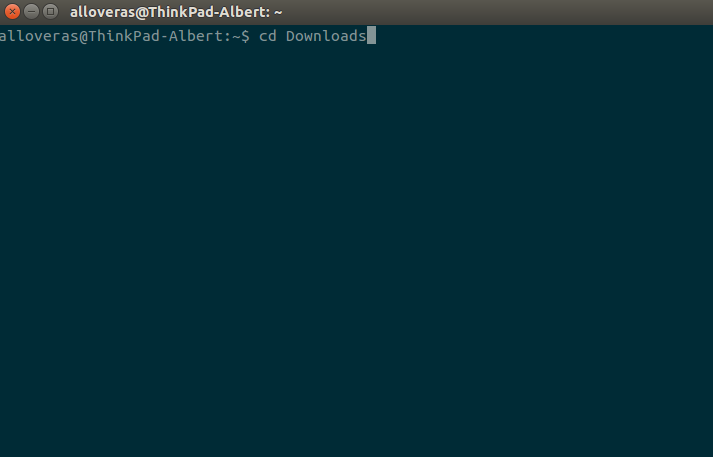
\includegraphics[scale=0.4]{img/Download_Folder_Move.png}
\end{center}

\noindent Un cop a la carpeta ens disposem a realitzar la configuració del codi font d'Allegro 5 per a que pugui ser compilat al nostre ordinador. Per fer-ho ens ajudarem d'una eina que hem instal·lat al començament del manual, concretament, \textbf{CMake}. Per fer-ho executarem la següent comanda:

\begin{center}
	\textbf{cmake CMakeLists.txt}
\end{center}

\newpage

\noindent Si tot va bé, al terminal començaran a realitzar-se comprovacions i configuracions que haurem d'esperar que finalitzin per poder procedir amb el procés d'instal·lació d'Allegro 5. A continuació és mostra un exemple gràfic del procés citat anteriorment:

\begin{center}
	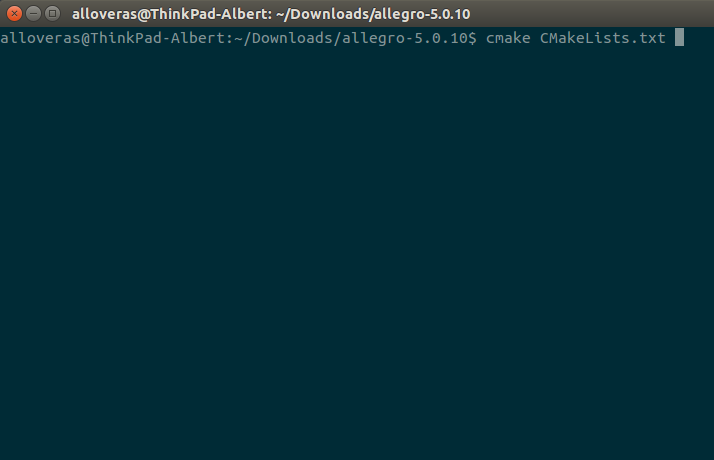
\includegraphics[scale=0.4]{img/CMake_CMakeLists.png}
\end{center}

\noindent Un cop executat la comanda el procés que hauria d'aparèixer al terminal hauria de ser el següent:

\begin{center}
	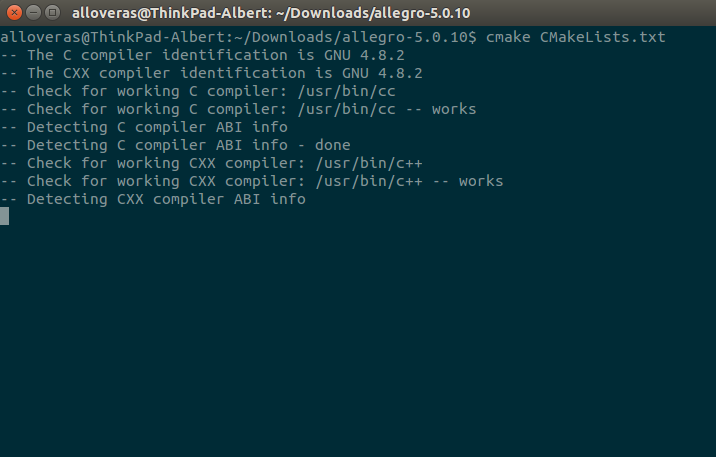
\includegraphics[scale=0.4]{img/CMake_Execution.png}
\end{center}

\noindent Un cop acabat el procés de configuració, haurem de realitzar la compilació del codi font. Per fer-ho, executarem al terminal la següent comanda:

\begin{center}
	\textbf{sudo make}
\end{center}

\noindent Al nostre terminal l'execució de la comanda \textbf{sudo make} s'hauria d'efectuar de la següent manera:
\begin{center}
	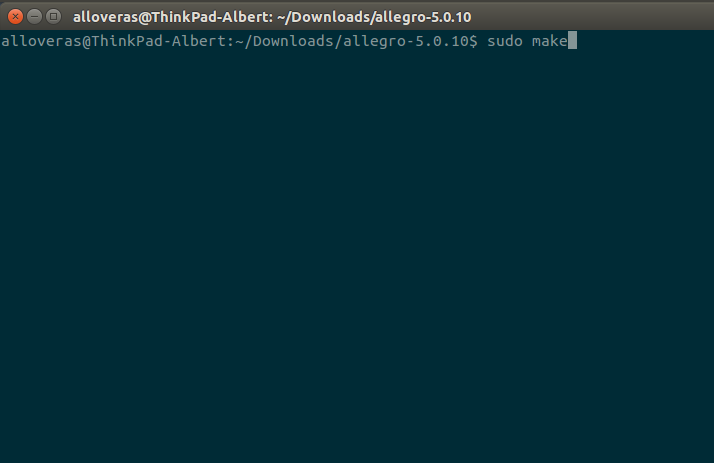
\includegraphics[scale=0.4]{img/Make_Command.png}
\end{center}

\noindent A continuació, mostrem un exemple gràfic del procés de compilació de les fonts d'Allegro 5:

\begin{center}
	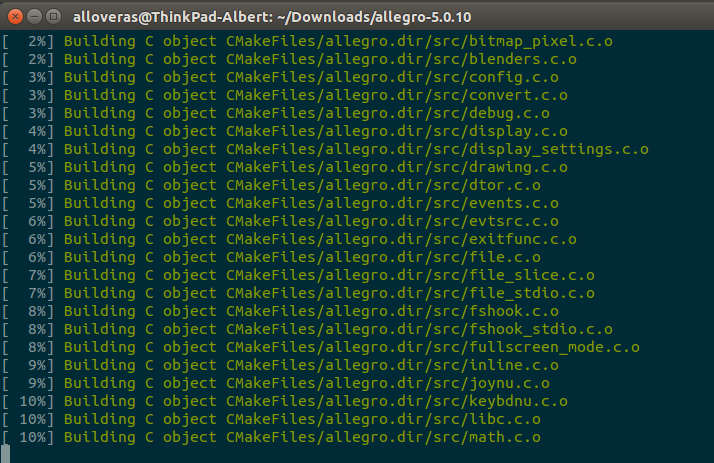
\includegraphics[scale=0.4]{img/Make_Process.png}
\end{center}

\noindent Un cop finalitzada la compilació, ja estem llestos per instal·lar definitivament els binaris compilats al nostre ordinador. Per fer-ho ens servirem de la comanda següent:

\begin{center}
	\textbf{sudo make install}
\end{center}

\noindent A continuació es deixa una imatge de la execució de la comanda citada anteriorment:
\begin{center}
	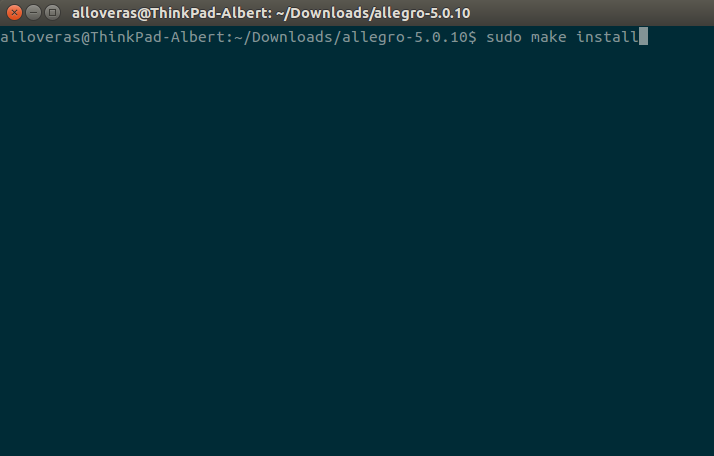
\includegraphics[scale=0.4]{img/Make_Install_Command.png}
\end{center}

\noindent L'execució de la comanda \textbf{sudo make install} hauria de produir el següent output al nostre terminal:

\begin{center}
	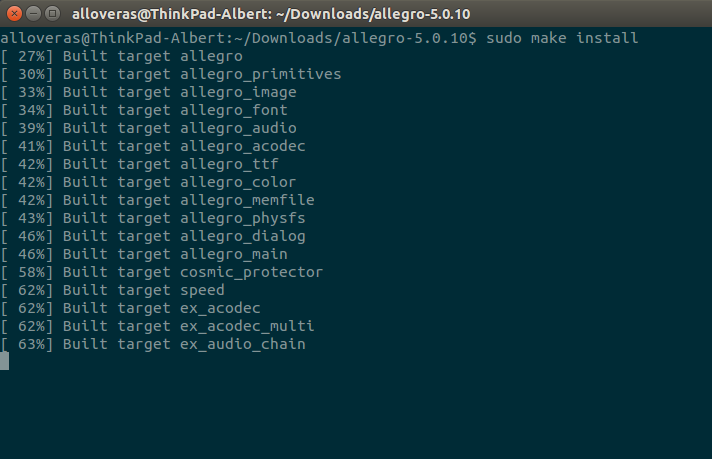
\includegraphics[scale=0.4]{img/Make_Install_Process.png}
\end{center}

\noindent Arribats a aquest punt, ja tenim Allegro 5 instal·lada al nostre ordinador. A partir d'ara ja podem usar la llibreria en qualsevol dels nostres projectes que requereixin d'interfícies gràfiques d'usuari. Només ens caldrà configurar l'IDE amb el que estiguem treballant per tal de que alhora de compilar pugui localitzar els fitxers i les dependències en qüestió de la pròpia llibreria. Aquest procés de configuració, s'explica amb tot detall al manual de configuració de Code-Lite + Allegro 5 que podreu trobar a l'eStudy.

\end{document}